\usetikzlibrary{arrows.meta}
\begin{frame}{HTTP typical flow}
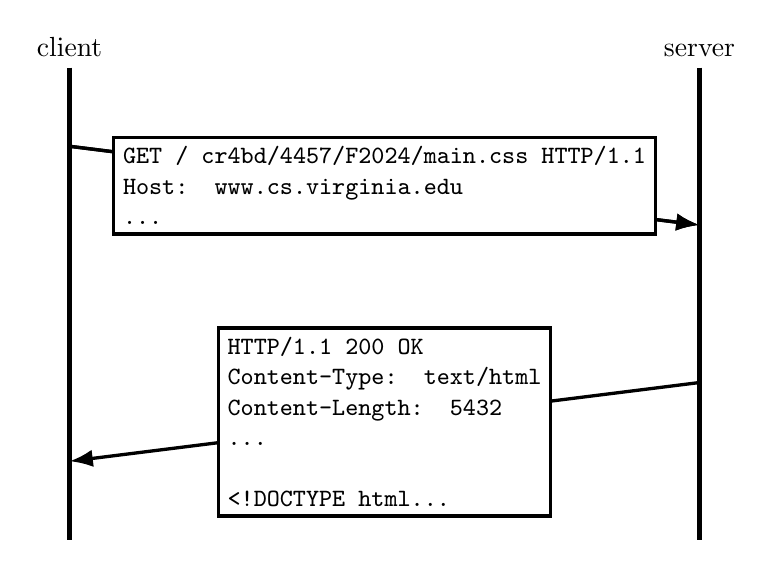
\begin{tikzpicture}
\tikzset{
    nodeline/.style={draw,ultra thick},
    msgline/.style={draw,very thick,-Latex},
    msgbox/.style={draw,fill=white,font=\small\tt,align=left},
}
\draw[nodeline] (0, 0) -- ++(0, -6) node[pos=0,above] {client};
\draw[nodeline] (8, 0) -- ++(0, -6) node[pos=0,above] {server};
\draw[msgline] (0, -1) -- (8, -2) node[midway,msgbox] {
    GET /~cr4bd/4457/F2024/ HTTP/1.1 \\
    Host: www.cs.virginia.edu \\
    \ldots
};
\draw[msgline] (8, -4) -- (0, -5) node[midway,msgbox] {
    HTTP/1.1 200 OK \\
    Content-Type: text/html \\
    Content-Length: 5432 \\
    \ldots \\
    ~ \\
    <!DOCTYPE html\ldots
};
\draw[msgline] (0, -1) -- (8, -2) node[midway,msgbox] {
    GET /~cr4bd/4457/F2024/main.css HTTP/1.1 \\
    Host: www.cs.virginia.edu \\
    \ldots
};
\end{tikzpicture}
\end{frame}

\begin{frame}{HTTP message fields}
\begin{itemize}
\item requests:
    \begin{itemize}
    \item method (GET, HEAD, POST, \ldots) --- what to do
    \item URI (`path' and `query' part of URL, usually)
    \end{itemize}
\item responses:
    \begin{itemize}
    \item status code and message (200 OK, 404 Not Found, etc.)
    \end{itemize}
\item both:
    \begin{itemize}
    \item headers (key-value pairs)
    \item (sometimes) message body (arbitrary data)
    \end{itemize}
\end{itemize}
\end{frame}

\begin{frame}{HTTP/1.1 message format (RFC 2616)}
\begin{itemize}
\item ASCII text over TCP or TLS 
\item all newlines use `CRLF' (\textbackslash0d\textbackslash0a = \textbackslash r\textbackslash n)
\end{itemize}
\providecommand{\crlf}{\textit{\color{black!50}CRLF}}
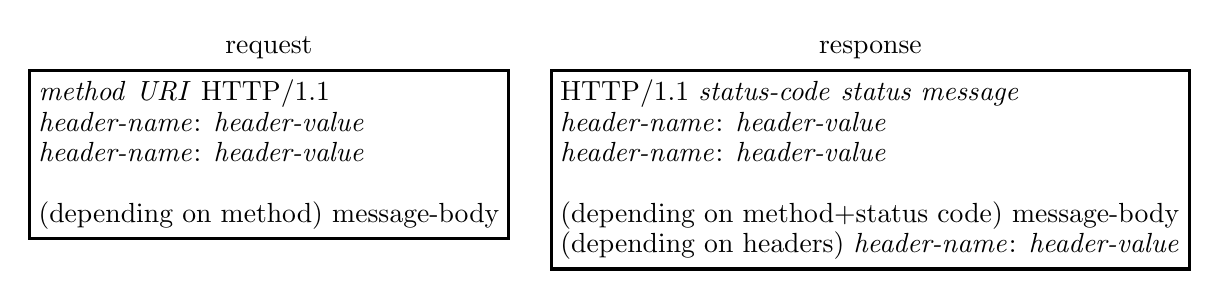
\begin{tikzpicture}
\node[draw,align=left,very thick,font=\fontsize{10}{11}\selectfont,label={north:request}] (request) {
\textit{method} \textit{URI} HTTP/1.1\\
\textit{header-name}: \textit{header-value} \\
\textit{header-name}: \textit{header-value} \\
~ \\
(depending on method) message-body
};
\node[anchor=north west,draw,align=left,font=\fontsize{10}{11}\selectfont,very thick,label={north:response}] 
at ([xshift=.5cm]request.north east){
HTTP/1.1 \textit{status-code} \textit{status message} \\
\textit{header-name}: \textit{header-value} \\
\textit{header-name}: \textit{header-value} \\
~ \\
(depending on method+status code) message-body \\
(depending on headers) \textit{header-name}: \textit{header-value}
};
\end{tikzpicture}
\end{frame}

\begin{frame}{HTTP/2, HTTP/3}
    \begin{itemize}
    \item `new' versions, not ubiquitously deployed
        \begin{itemize}
        \item HTTP/2: over TCP \textit{or} over TLS over TCP
        \item HTTP/3: over QUIC over UDP
        \end{itemize}
    \vspace{.5cm}
    \item multiple `streams' within one connection 
    \item send series of `frames' with stream ID + type + data
    \item frame types include:
        \begin{itemize}
        \item HEADERS --- encode message headers (key/value pairs)
        \item DATA --- include message bodies
        \end{itemize}
    \item method, status-code, URI encoded as special headers
    \end{itemize}
\end{frame}

\begin{frame}{HTTP/1.1 example (GET)}
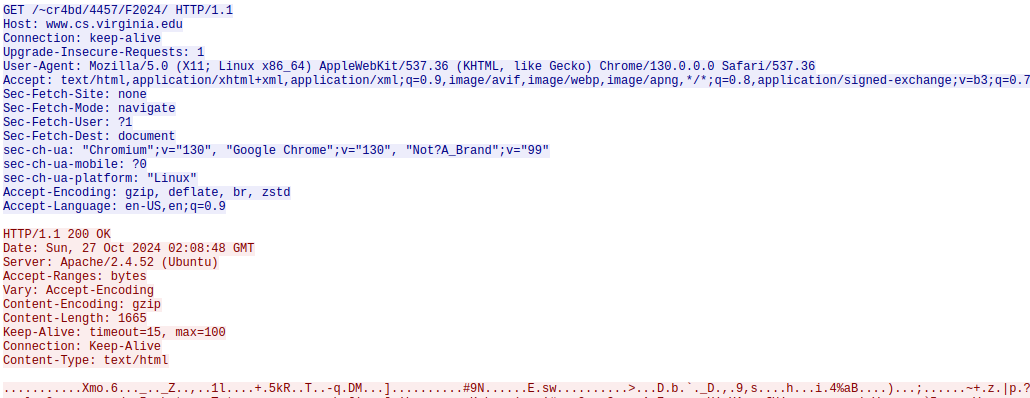
\includegraphics[width=\textwidth]{../http/http-wireshark-simple}
\end{frame}

\begin{frame}{HTTP/2.0 example (GET request)}
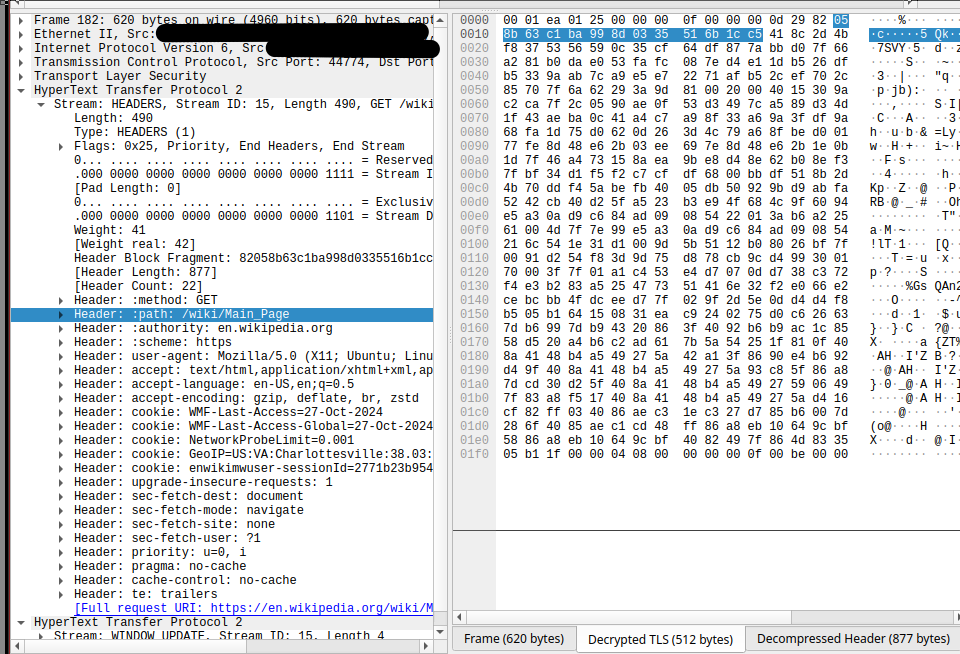
\includegraphics[width=\textwidth]{../http/http2-get-ex}
\end{frame}

% FIXME: HTTP/2.0 response

\begin{frame}{HTTP/1.1 example (POST)}
% FIXME
\end{frame}
